\chapter[Practical and Secure Location Verification for Payments]{Practical and Secure Location Verification Tokens for Payments}
\label{chap:ps_tee}

\section{Introduction}

Fraudulent transactions at points of sale made with stolen or duplicated payment
cards are a major problem.  In 2010 alone, these transactions constituted one
third of the 1.26 billion EUR total fraud in the Single Euro Payments
Area~\cite{ECB2012}. To improve the security of existing payment systems,
companies and researchers have suggested usage of mobile devices as a
two-factor authentication mechanism~\cite{mastercardpatent, park09acsac}. As
most users already have smartphones, deployment of such two-factor
authentication is practical. Many online service providers already employ
two-factor authentication using smartphones.  Examples of this approach are
online banking applications~\cite{barclays_pinsentry} and Google 2-Step
Verification~\cite{google_authentication}.  In a typical implementation, the
user reads a one-time code off the smartphone screen and enters it on
the service's web page during login.  Login operations to services like online
banking are typically performed when the user has time to interact with his
smartphone to complete the authentication process. In addition, web services are
easily modifiable. Thus, in most cases, an extra authentication step can be
added to the login procedure of a web service at little cost. This approach
cannot be, however, integrated in point of sale transactions, because
interactions at a shop counter with a smartphone are inconvenient and add
undesirable transaction delay. Additionally, the payment terminal infrastructure
is hard to modify.

Recent proposals leverage location data from the user's phone as the second
authentication factor for payments~\cite{mastercardpatent,park09acsac}. During a
transaction, either the card issuer~\cite{mastercardpatent} or the
user~\cite{park09acsac} can verify that the location of the user's smartphone
matches the location of the point of sale terminal used for the transaction.
Previous work, however, overlooks important usability and security aspects, as
it requires changes in both the point of sale infrastructure and the user
experience. Furthermore, it assumes a trustworthy mobile OS, even though
compromise of mobile operating systems has become
commonplace~\cite{Felt11,zhou2012sp}.

To secure mobile services despite mobile OS compromise, researchers have
proposed using system-wide Trusted Execution Environments (TEEs), such as ARM
TrustZone~\cite{ARMTrustZone}, which provide isolated execution of applications
and secure storage of
credentials~\cite{sariou10hotmobile,liu12mobisys}. Integrating system-wide TEEs
with any two-factor authentication protocol, however, requires the verifying
party (e.g., the card issuer) to correctly bind a user's identity to the TEE
running on his mobile device through an enrollment scheme. How to establish this
binding in the presence of a compromised OS is an open
problem~\cite{2013_spsm_marforio}.

In this chapter we propose a smartphone-based two-factor authentication
solution for payments at points of sale that uses location data to identify
fraudulent transactions.  In contrast to previous work, our solution does not
require changes to established user interaction models and is compatible with
the existing point of sale infrastructure.  We leverage system-wide TEE
architectures to provide a secure system, despite mobile OS compromise.  As part
of our solution, we design two secure enrollment schemes for smartphones to
bootstrap two-factor authentication for payments, which may also be used in
other application scenarios. To summarize, We make the following contributions.

\begin{itemize}
\item We propose a smartphone-based two-factor authentication solution for
  payments at points of sale, that uses the phone's location as the second
  authentication factor. Our solution makes use of smartphone TEEs to resist
  mobile OS compromise.
\item As part of our solution, we construct two secure enrollment schemes that
  allow a card issuer to bind the identity of a user with the TEE running on his
  device. The first enrollment scheme leverages the unique identity of the
  user's SIM card and resists adversaries that can remotely compromise the
  victim's mobile OS. The second enrollment scheme uses specially crafted SMS
  messages that are processed within the device baseband OS. This scheme
  provides protection against more powerful adversaries that can additionally
  perform hardware attacks on devices to which they have physical access.
\item Through prototype implementation using an open-source baseband OS, Android
  devices, and an ARM TrustZone development board, we show that our solution can
  be easily deployed. It requires small changes to existing smartphones, and no
  changes to the point of sale infrastructure and the user experience. Our
  experiments show that, during a transaction, location verification takes less
  than 4 seconds on average, which is a tolerable delay for most payment
  scenarios.
\item We survey known approaches for two-factor authentication using mobile
  phones and argue why they cannot be deployed in the considered application
  scenario. We also analyze commonly suggested enrollment schemes and show why
  they do not withstand strong attackers that we consider in this work.
\end{itemize}

\section{Problem Statement}
\label{sec:ps_tee_problem}

Our goal is to design a smartphone-based two-factor authentication mechanism
that prevents fraudulent transactions at points of sale.  In the following we
detail the requirements for any deployable and secure solution to this
problem.

We first aim to design mechanisms that must not change the user interaction
model and the current point of sale infrastructure.  Previous work shows that
introducing changes to established user interaction models makes adoption of new
security mechanisms impractical~\cite{bonneau12sp}.  Similarly, having to update
the deployed points of sale makes adoption of additional security mechanisms
hard~\cite{Guida04}.

Second, a solution must remain secure despite a targeted adversary that may
compromise the mobile OS on the victim's device.  Current
systems~\cite{barclays_pinsentry, google_authentication} and related research
proposals~\cite{czeskis12ccs, Mannan11}, which use smartphones for two-factor
authentication, assume the mobile OS to be trustworthy.  This assumption is too
strong, as the complexity of smartphone platforms has increased, mobile
operating system vulnerabilities have become commonplace~\cite{Felt11,
  zhou2012sp}.

Third, any two-factor authentication mechanism that replaces dedicated tokens
with smartphones, must have an enrollment scheme, where the verifying
party binds the identity of a user to his device.  A dedicated security token is
a user-specific device, which the service provider binds to the user identity
before the token is shipped to the user. As smartphones replace such tokens, the
service provider can only bind the user identity to his device after the user
has already purchased the smartphone. In addition to initial enrollment, a
practical solution must also support device migration. In applications like
payments at points of sale, it is realistic to assume a one-time service
registration performed, for example, when the user visits a branch of his bank
in person. Requiring a similar operation every time the user starts using a new
smartphone becomes both expensive for the bank and inconvenient for the user.

\section{Background on TrustZone-enabled Smartphones}
\label{sec:ps_tee_mobile}

\begin{figure}[!ht]
    \centering
    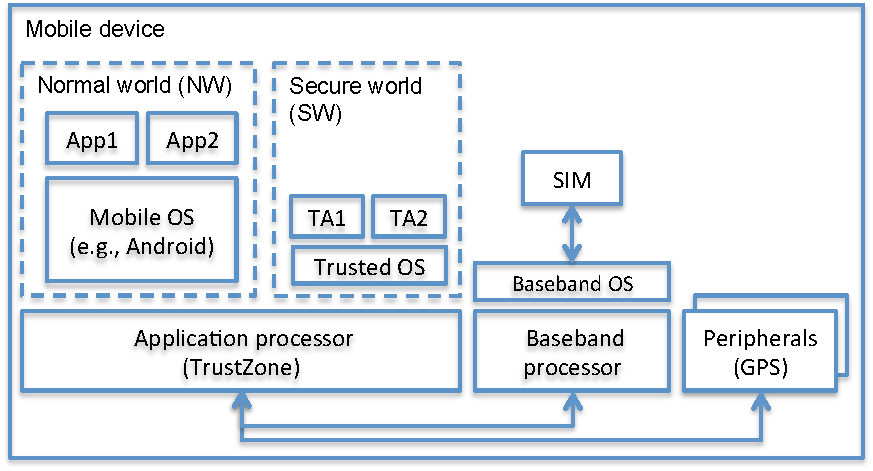
\includegraphics[width=.9\linewidth]{figures/phonesecures/tee_mobile}
    \caption[Architecture overview of a TrustZone-enabled device]{Architecture overview of a TrustZone-enabled device.}
    \label{fig:ps_tee_mobile}
\end{figure}

Most mobile devices support system-wide TEEs, like ARM
TrustZone~\cite{ARMTrustZone}. In a TrustZone-enabled device, the application
processor supports two execution states, namely, \emph{secure world} and
\emph{normal world} (or non-secure world). The processor switches between these
states in a time-slicing manner, so that only one state is active at a time.
The normal world runs the mobile OS and regular applications on top of it. The
secure world runs \emph{trusted applications} (TAs), which are executed on top
of a small layer of software called the \emph{trusted OS}. The overview of the
architecture of a TrustZone-enabled mobile device is shown in
Figure~\ref{fig:ps_tee_mobile}.

In general the security extensions that are implemented in an ARMv7 system-on-chip make it seem as if there were two virtual CPUs running on a single physical core. Figure~\ref{fig:ps_tz_cores} shows the details of the security extensions implemented in the CPU core. Processors that support security extensions must provide: two separate virtual Memory Management Units (MMUs) two separate Virtual Memory Address spaces for both worlds; an additional processor mode (the \emph{monitor} mode); a new instruction (\texttt{SMC} --- secure monitor call) to switch to monitor mode; banked and common coprocessor configuration registers; and finally, the possibility to tag cache lines as secure and non-secure.

\begin{figure}[!ht]
    \centering
    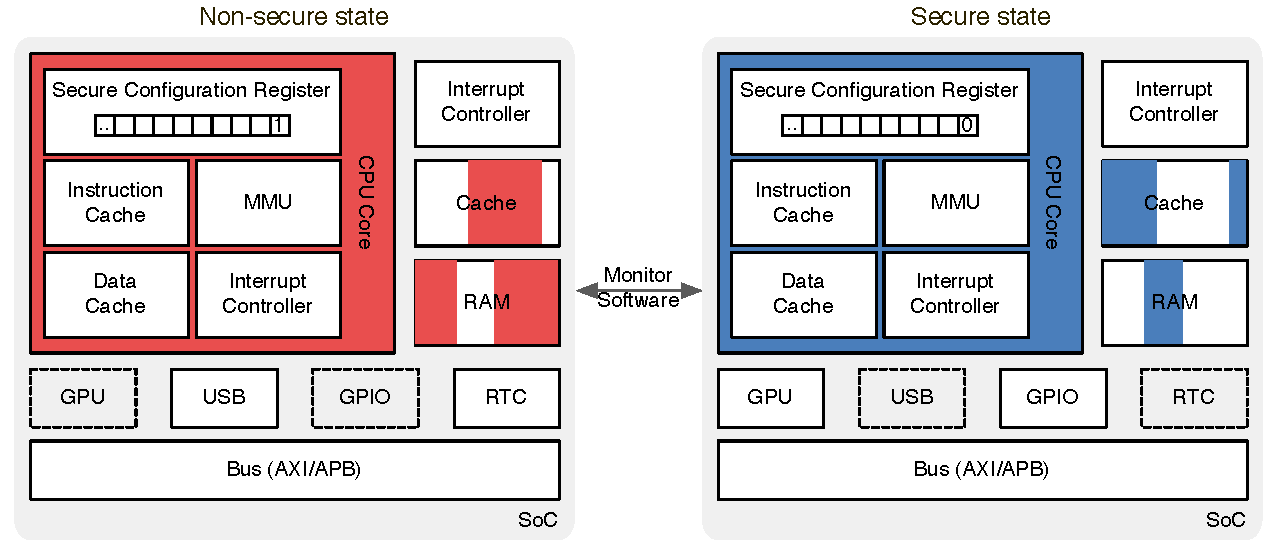
\includegraphics[width=1\linewidth]{figures/phonesecures/tee_tz_cores}
    \caption[TrustZone-enabled SoC cores in Non-secure and Secure states]{Sample configuration for a TrustZone-enabled SoC with virtual cores in the Non-secure and Secure state.}
    \label{fig:ps_tz_cores}
\end{figure}

Applications in the secure world are isolated from the mobile OS in the normal
world. In contrast to dedicated security elements like smart cards and TPMs,
system-wide TEEs like TrustZone allow secure access to various device hardware
resources from the TEE, and to configuration of secure mobile device event
handling. Access to device peripherals and the baseband processor environment
is typically possible by both the trusted OS in the secure world and the mobile
OS in the normal world. In addition, certain peripherals can be reserved for
secure world access only. Access to memory areas can be configured in a similar
manner, and in a mobile device a small amount of memory is reserved for the
secure world. Access control to hardware resources is implemented through
specific control hardware and signals on the system communication bus.

This separation is enabled in a TrustZone-aware device by augmenting some system components. In particular, as seen in Figure~\ref{fig:ps_tz_internal}, the system supports external memory isolation through the TZASC (TrustZone Access Space Controller), internal memory isolation through the TZMA (TrustZone Memory Adapter), an AXI-to-APB Bridge (Advance eXtensible Interface to Advanced Peripheral Bus) to connect low-bandwidth peripherals, and the TZPC (TrustZone Protection Controller) to configure the TZMA adapter.

\begin{figure}[!ht]
    \centering
    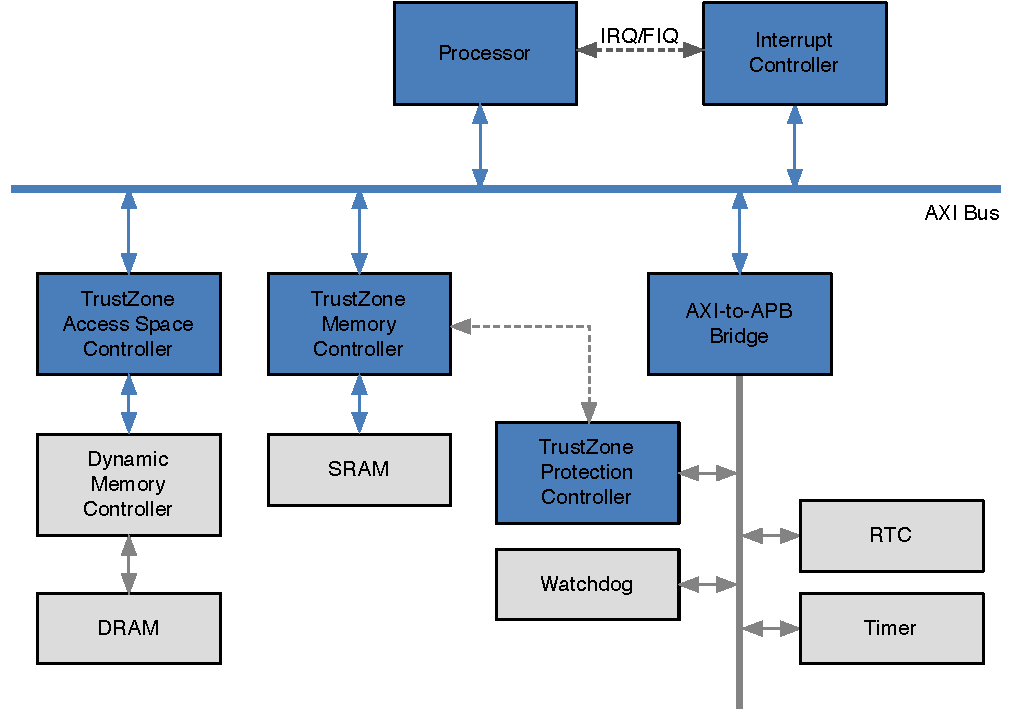
\includegraphics[width=.9\linewidth]{figures/phonesecures/tee_tz_internal}
    \caption[TrustZone-aware components in an example ARM system design]{TrustZone-aware components (highlighted in blue) in an example ARM system design.}
    \label{fig:ps_tz_internal}
\end{figure}

Hardware interrupts can also be configured for secure world processing if need be. For more details on TrustZone, we advise the interested reader to look at the ARM documentation~\cite{ARMTrustZone}.

A standard trusted OS only allows execution of code that has been signed by a
trusted authority, such as the device manufacturer. Typically, the device
manufacturer ships each device with a device-specific key-pair (we refer to it
as the \emph{device key}). The public part of the device key is certified by the
manufacturer, and the issued \emph{device certificate} contains an immutable
device identifier, such as the IMEI number (International Mobile Equipment
Identity).  The corresponding private key is only accessible by software that
runs in the secure world~\cite{kostiainen2011codaspy}.

To limit the size of the TCB, a typical trusted application handles only
security-critical processing, such as user credential processing or data
encryption. A \emph{companion application}, running in the normal world, handles
the communication, the UI rendering and other complex tasks.  The rationale is
that inclusion of complex libraries in the trusted OS, like network stacks or
video drivers, considerably increases the size of the device TCB, and with that
the attack surface of the secure world.

Device manufacturers have shipped their mobile devices with system-wide TEEs
like ARM TrustZone for almost a decade.  The usage of these environments, thus
far, has been primarily limited to a few manufacturer-specific use cases, like
implementation of subsidy locks and secure boot~\cite{kostiainen2011codaspy}.
Deployment of third-party applications in system-wide TEEs has been limited,
because the installation of new trusted applications is subject to the approval
of the device manufacturer.  Nevertheless, recent research shows that
system-wide TEEs can be safely opened up for third-party trusted application
development~\cite{kostiainen09asiaccs}, and on-going TEE API standardization
activities~\cite{globalplatformspecs} are likely to make trusted application deployment more
accessible to third-parties.

\section{Adversarial Model}
\label{sec:ps_tee_adv}

We consider a targeted adversary who possesses the victim's payment card (or a
clone) and knows its PIN code (if any).  His goal is to perform a fraudulent
transaction at a point of sale.  The adversary does not have physical access to
the victim's smartphone.  He does, however, have access to other similar
devices.  We regard the device hardware, the trusted OS and the baseband OS as
the TCB on the victim's device, and distinguish between two types of adversary.

\begin{figure}[!ht]
    \centering
    \subfigure[Victim's device]{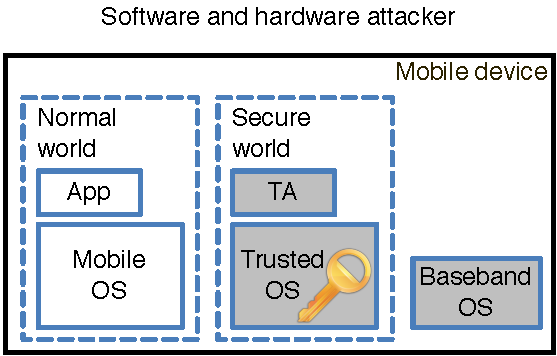
\includegraphics[width=.5\columnwidth]{figures/phonesecures/tee_adversary_a}}
    
    \subfigure[Adversary's device]{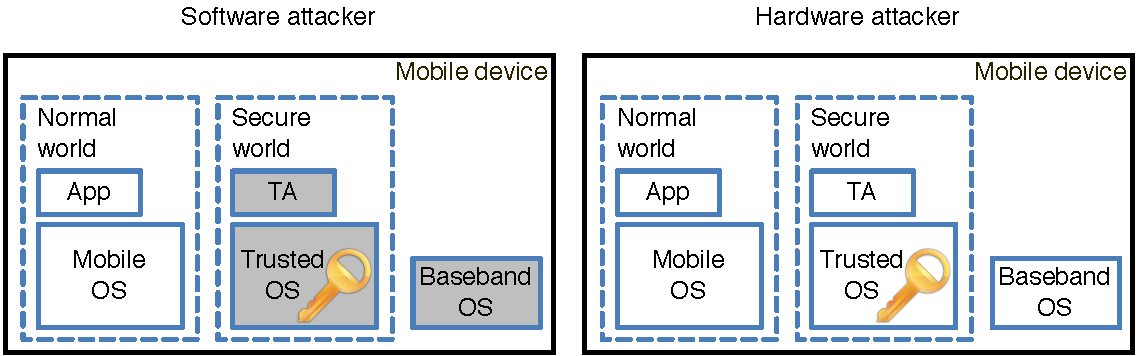
\includegraphics[width=1\columnwidth]{figures/phonesecures/tee_adversary_b}}
    
    
    % 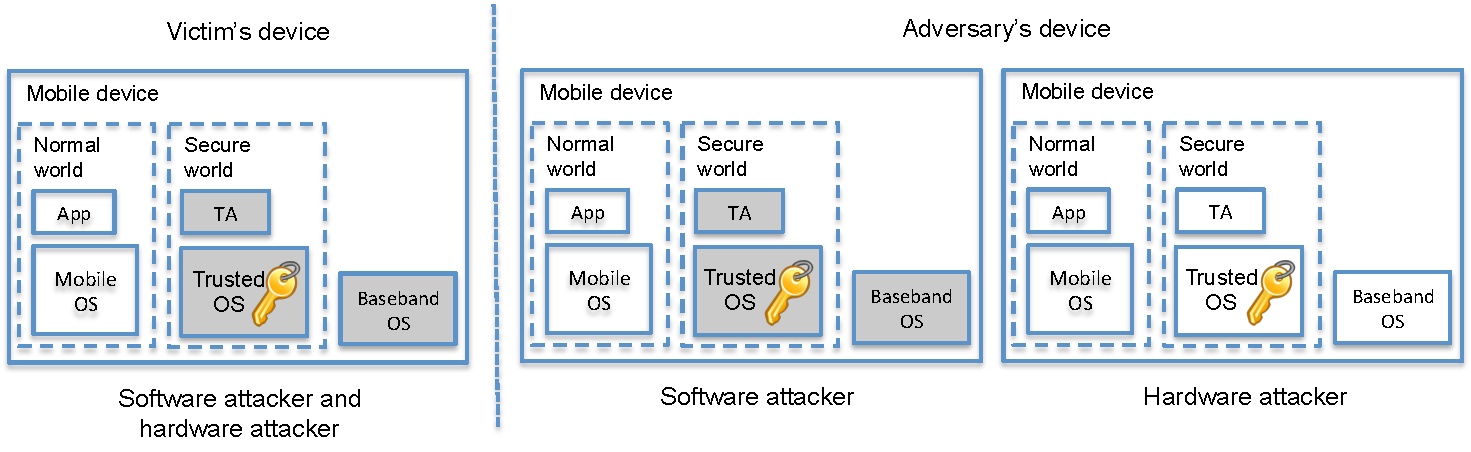
\includegraphics[width=\linewidth]{figures/phonesecures/tee_adversary}
    \caption[Adversarial models for a TrustZone-enabled smartphone]{Adversarial model. Grey boxes show trusted components for each type
      of adversary. The victim's device (a) can be only targeted with
      remote attacks and the TCB is the same in both attacker models. Trusted
      components on the adversary's device (b) depend on the
      considered attacker model: a software attacker cannot tamper with the TCB
      on his device; a hardware attacker has complete access to any component
      of his device.}
    \label{fig:ps_tee_adversary-model}
\end{figure}

A \emph{software} attacker can remotely compromise the mobile OS on the victim's
smartphone, but cannot compromise its TrustZone secure world nor the baseband OS
execution.  Likewise, he cannot compromise the TrustZone secure world nor the
baseband OS on any other device.  Software attacks against the mobile OS are a
real threat~\cite{Felt11,zhou2012sp}, while software attacks against the TCB
(i.e., the baseband OS and the TrustZone secure world) are significantly harder,
due to its limited size and attack surface.

A \emph{hardware} attacker can additionally perform hardware attacks against
devices that he owns or has physical access to.  On such devices, he may
compromise the baseband OS execution, the TrustZone secure world and,
ultimately, extract the TrustZone-protected secrets, such as the device key.
This adversarial model is justified by the fact that neither a TrustZone-enabled
processor nor the baseband processor provide tamper resistance properties,
commonly found in smart cards or hardware security
modules. Figure~\ref{fig:ps_tee_adversary-model} illustrates trusted software
components (gray boxes) in these different scenarios.

Neither of the attackers controls the cellular network
communication. Furthermore, they cannot launch GPS spoofing attacks on the
victim's device. Finally, we do not address denial-of-service attacks.

\section{Our Solution}
\label{sec:ps_tee_architecture}

We use the location of the user's phone as the second authentication factor
during a transaction at a point of sale.  Our solution leverages system-wide
TEEs available on mobile devices to provide card issuers with trustworthy
location information despite a potentially compromised mobile OS on the user's
smartphone.  We focus on ARM TrustZone since it is currently the most widely
deployed system-wide TEE on mobile devices.  The schemes we propose can,
nevertheless, be used with other system-wide TEEs as well.

\begin{figure}[!ht]
    \centering
    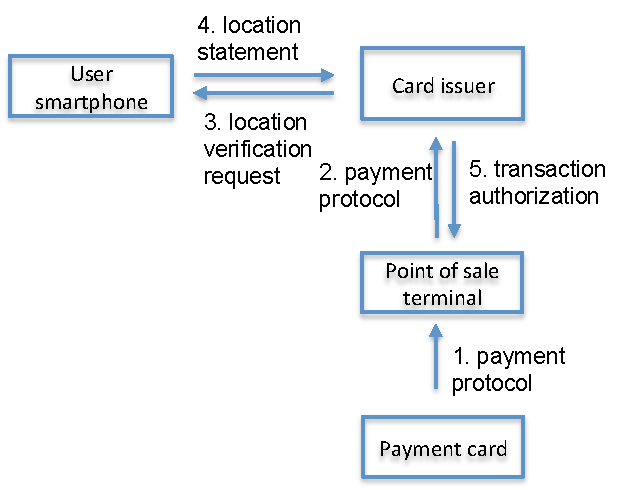
\includegraphics[width=.8\linewidth]{figures/phonesecures/tee_overview}
    \caption[Overview of location-based two-factor authentication for
      payments at point of sale]{Overview of location-based two-factor authentication for payments at point of sale. During a payment transaction, the card issuer
      queries the user's smartphone for its location over an Internet
      connection.}
    \label{fig:ps_tee_overview}
\end{figure}

Figure~\ref{fig:ps_tee_overview} shows an overview of our scheme. Prior to payments at a point of sale, we assume that the user has already installed two applications
provided by the card issuer on his device: a companion application running in
the normal world and a trusted application running in the secure world.
Additionally, the user has also completed an enrollment scheme (see below), and
the card issuer has established a binding between the user and the TEE on his
device.  During payment, the user inserts or swipes his payment card in a point
of sale terminal and optionally enters its PIN code (step 1). The terminal sends
the transaction information to the card issuer (step 2). The card issuer
contacts the TEE on the user's smartphone (step 3), which replies with a
location statement (step 4). The card issuer then checks whether the location
statement was sent by the correct device and compares it against the location of
the terminal. Finally, the card issuer sends the transaction decision (authorize
or deny) to the terminal (step 5).

We leverage location data due to two main reasons.  First, we want a solution
that does not change the user interaction model and the hardware infrastructure
(see Section~\ref{sec:ps_tee_problem}). We therefore resort to the sensing capabilities
of modern smartphones. Second, among available smartphone sensors, GPS units are
almost ubiquitous, and previous work has shown that GPS coordinates are a
practical and useful means that card issuers can leverage to identify fraudulent
transactions~\cite{mastercardpatent,park09acsac}. Our solution could, in
principle, use any sensor available on the device.

\subsection{User Enrollment}
\label{sec:ps_tee_enrollment}

Before the card issuer can verify the location of the user's smartphone, it
needs to bind the user identity to the TEE running on his mobile device.  To
achieve this binding, we present two enrollment schemes.  The \emph{signed-IMSI
  enrollment} scheme is easier to deploy but can only withstand software
attackers; the \emph{baseband-assisted enrollment} scheme is also secure against
hardware attackers. However, the latter requires minor software changes to the baseband
OS.  Both schemes leverage the implicit binding between the user and his SIM
card.  They require a one-time registration in which the user provides his phone
number to the card issuer in a reliable manner, for example, by visiting his
bank's branch in person.  The goal of both enrollment schemes is to establish a
shared \emph{service key}, between the card issuer and the trusted application
running in the TEE on the user's device.

\paragraph{Signed-IMSI enrollment.}

The card issuer uses the SIM identifier (i.e., the IMSI) and the mobile network
infrastructure to verify that the enrolling device is indeed the one where the
user's SIM card is installed. Figure~\ref{fig:ps_tee_enrollment-trustzone} illustrates the steps of the enrollment scheme.

\begin{figure}[!ht]
    \centering
    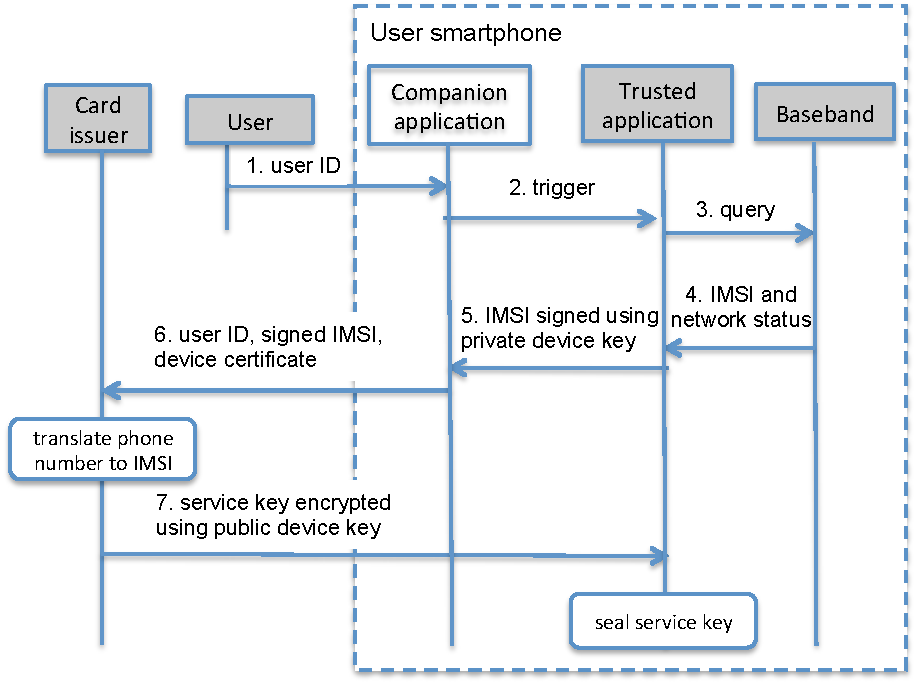
\includegraphics[width=\linewidth]{figures/phonesecures/tee_enrollment-trustzone}
    \caption[Signed-IMSI enrollment scheme]{Signed-IMSI enrollment scheme.
    Gray boxes are trusted entities. The trusted application fetches the IMSI
    of the installed SIM card from the baseband processor. It signs the IMSI
    with the private device key and forwards it to the card issuer (through the
    companion application). The card issuer can link the IMSI to a previously
    registered phone number.}
    \label{fig:ps_tee_enrollment-trustzone}
\end{figure}

The user starts the companion application and provides his user ID, (e.g., the
bank customer number, step 1). This application triggers the execution of the
trusted application (step 2) that queries the baseband OS for the IMSI of the
SIM card (steps 3-4).\footnote{The IMSI is needed for cellular protocols and is
available to the baseband OS through standardized interfaces.} The trusted
application also verifies from the baseband OS that the device is connected to
the mobile network, to discard the possibility of a fake SIM card reporting a
false IMSI.\footnote{A false SIM card lacks the correct keying material to
connect to the cellular network} The trusted application signs the IMSI using
its device private key (step 5) and passes the signature to the companion
application. At this point the companion application sends the signed IMSI, the
user ID, and the device certificate to the card issuer over the Internet (step
6). The card issuer uses the received user ID to retrieve the user's phone
number and queries the mobile infrastructure for the corresponding IMSI (see
Section~\ref{sec:ps_tee_implementation} for details). The card issuer checks
that the IMSI received from the user's phone matches the one reported by the
mobile infrastructure. If the two IMSIs match, the card issuer proceeds to
verify (\emph{i}) the validity of the device public key using the device certificate
and the public key of the manufacturer, and (\emph{ii}) the validity of the signature
over the IMSI. If all checks are successful, the card issuer picks a fresh
service key and encrypts it under the device public key; the ciphertext is sent
to the user's smartphone (step 7). The companion application passes the
encrypted service key to the trusted application that decrypts it using the
private part of the device key and encrypts it using a symmetric storage key
available only in the secure world (\emph{sealing}). The sealed service key can
be stored by the companion application in the normal world.

\paragraph{Baseband-assisted Enrollment.}

\begin{figure}[!ht]
    \centering
    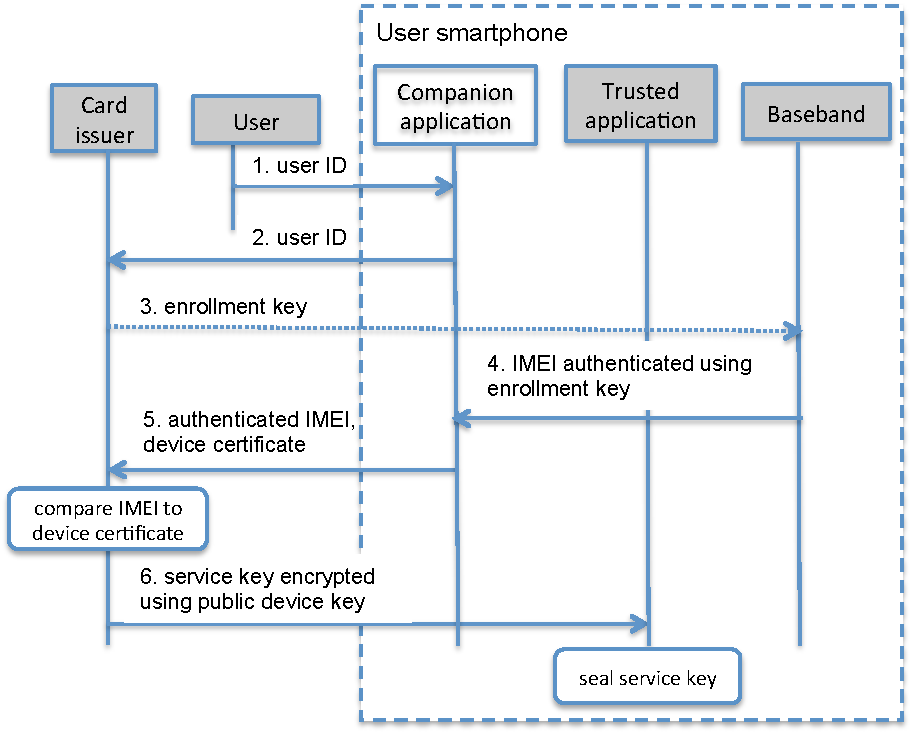
\includegraphics[width=\linewidth]{figures/phonesecures/tee_enrollment-baseband}
    \caption[Baseband-assisted enrollment scheme]{Baseband-assisted enrollment
    scheme. Gray boxes are trusted entities. The card issuer sends an SMS
    message with an enrollment key (dotted line); the baseband OS uses that key
    to authenticate the device's IMEI and deletes the key. The card issuer can
    check the authenticated IMEI against the one received in the device
    certificate.}
    \label{fig:ps_tee_enrollment-baseband}
\end{figure}

In this scheme the card issuer sends an SMS message carrying an
\emph{enrollment key} to the phone number provided by the user during
registration. We augment the baseband OS to use this key and compute an
authentication tag on the device's IMEI.\footnote{The IMEI is bound to the
device key by the device certificate.} The steps of this scheme are shown in
Figure~\ref{fig:ps_tee_enrollment-baseband}.

The user starts the companion application and provides his user ID (step 1),
which is forwarded to the card issuer over the Internet (step 2). The card
issuer sends an enrollment SMS message to the corresponding user's phone
number, containing a fresh enrollment key (step 3). The baseband OS on the
user's device intercepts the SMS message and extracts the enrollment key. The
baseband OS uses the enrollment key to authenticate the device's
IMEI,\footnote{The IMEI is read from a read-only memory on the device, written
by the device manufacturer. The baseband OS has access to the IMEI to handle
cellular communication.} provides the authentication tag to the companion
application (step 4), and deletes the enrollment key. The companion application
forwards the authenticated IMEI and the device certificate to the card issuer
(step 5). The card issuer checks (\emph{i}) the validity of the device certificate,
(\emph{ii}) the validity of the authentication tag, and (\emph{iii}) that the IMEI
authenticated with the enrollment key matches the one in the received
certificate. If all checks are successful, the card issuer picks a fresh
service key and encrypts it under the device public key extracted from the
device certificate; the ciphertext is sent to the user's smartphone (step 6).
The companion application passes the encrypted service key to the trusted
application that seals it.

\subsection{Location Verification}
\label{sec:ps_tee_locationverification}

\begin{figure}[!ht]
    \centering
    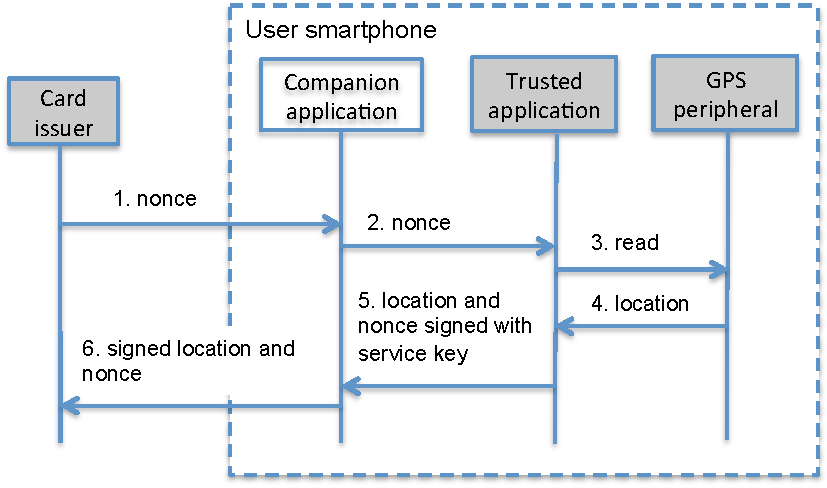
\includegraphics[width=0.95\linewidth]{figures/phonesecures/tee_verification}
    \caption[Location verification is a challenge-response protocol using the
    service key established during enrollment]{Location verification is a
    simple challenge-response protocol using the service key established during
    enrollment. Gray boxes are trusted entities. The card issuer sends a nonce;
    the trusted application reads the GPS coordinates and authenticates them
    together with the nonce.}
    \label{fig:ps_tee_verification}
\end{figure}

After successful enrollment, the user's device shares a service key with the
card issuer that can be used to create an authentic channel between the two
parties. During a transaction payment, therefore, the card issuer can query the
device for an authenticated location statement. As detailed in
Figure~\ref{fig:ps_tee_verification}, the location verification is a simple
challenge-response protocol.

The card issuer picks a fresh nonce (for replay protection) and sends it to the
trusted application through the companion application (steps
1-2).\footnote{Alternatively, the card issuer could verify the freshness of
  location statements checking the timestamp provided by the GPS unit. As one of
  our goals is not to change the payment transaction user experience, the
  location verification must be initiated by the card issuer. Thus, a location
  verification requires the exchange of two messages between the card issuer and
  the user smartphone in either cases (i.e., usage of the GPS timestamp does not
  allow a more efficient implementation).}  The trusted application reads the
location coordinates from the device GPS unit (steps 3-4), unseals the service
key and uses it to authenticate the nonce and the current coordinates. The
authenticated message is sent back to the card issuer through the companion
application (steps 5-6).  The card issuer verifies the authenticity of the
location statement using the service key. At this point, the card issuer matches
the location of the user's smartphone against the one of the terminal used for
the transaction, to decide whether to authorize or deny the transaction.

We note that neither the companion application nor the trusted application need
to be continuously running in the background. The execution of the trusted
application is triggered by the companion application which, in turn, is started
by the mobile OS when receiving a request for that application (e.g., through a
push notification).

\subsection{Device Migration}

Both enrollment schemes support device migration by re-running the enrollment
operation. When the user switches to a new device and moves his SIM card to it,
he can start the enrollment process from the companion application of the new
device. As a result of either the signed-IMSI or the baseband-assisted
enrollment, the card issuer invalidates the previously used service key,
re-associates the user identity to the device key of the new device, and sends a
fresh service key to the TEE on that device. Device migration does not require
out-of-band communication with the card issuer as long as the user keeps his
phone number (even if he gets a new SIM card associated with his old phone
number).

\section{Security Analysis}
\label{sec:ps_tee_analysis}
		
Recall that our adversary holds the victim's payment card (or a clone) and his
goal is to make fraudulent transactions at points of sale. The adversary does
not have physical access to the victim's smartphone but he does have remote
control over that smartphone's mobile OS.

With the deployment of our system, the adversary must convince the card issuer
that the enrolled user's smartphone is close to the terminal where the
fraudulent transaction is taking place. To do so, the adversary must either
succeed in an impersonation attack during enrollment or tamper with the location
verification protocol.\footnote{We acknowledge that the adversary may still
  succeed in his goal if the fraudulent transaction takes place close to where
  the victim's device is located.}

In an impersonation attack, the adversary must halt the enrollment scheme on the
victim's device (he can do so since he controls that device's mobile OS), and
use the victim's ID to run the enrollment scheme on a device that he owns. In
particular, the adversary has two possible \emph{strategies}: he must induce the
card issuer to encrypt the service key either

\begin{itemize}
\item[(a)] under the public key of the adversary's device (the adversary will
  thus be able to make fraudulent transactions if his phone is in proximity of
  the terminal where the transaction takes place), or
\item[(b)] under a public key for which the adversary knows the private key (so
  that the adversary will be able to generate arbitrary location statements when
  the card issuer requests them).
\end{itemize}

In the following we provide an informal analysis of the enrollment schemes, with
respect to the two strategies above. Finally, we argue that the location
verification mechanism is secure after successful user enrollment.

\subsection{Signed-IMSI enrollment}

This enrollment scheme is secure against a software attacker as defined in
Section~\ref{sec:ps_tee_adv}.  This attacker can control the mobile OS on any device
(including the victim's) but does not have sufficient capabilities to control
any baseband OS or the TrustZone secure world execution environment.

Strategy (a) requires the adversary to start an enrollment scheme on his device
using the victim's ID.  Since the card issuer knows the victim's phone number
and can retrieve the corresponding IMSI, the adversary must force the trusted
application on his device to send the IMSI of the victim's SIM card.  To do so,
the adversary may use a custom SIM card where he can manipulate the IMSI.
However, such SIM card misses the key that the victim's SIM card uses for
authentication with the network operator and, thus, cannot connect to the
cellular network.  When the trusted application on the adversary's device
queries the baseband OS for cellular network status, it detects that the phone
is not connected and will abort the enrollment scheme.

Strategy (b) requires the adversary to hold a private key corresponding to a
valid (i.e., certified by the device manufacturer) public key. This is not
possible since a software adversary cannot compromise the ARM TrustZone
architecture of any device and leak the secrets stored therein.

\subsection{Baseband-assisted Enrollment}

This enrollment scheme is secure against a hardware attacker, as defined in
Section~\ref{sec:ps_tee_adv}, that controls the mobile OS on any device (including the
victim's), as well as the baseband OS and the TrustZone secure world execution
environment on devices to which he has physical access.

Strategies (a) and (b) require the adversary to either intercept the enrollment
SMS message and extract the enrollment key, or provide a crafted IMEI to the
baseband OS on the victim's device.  Since the adversary does not control the
GSM network, SMS messages cannot be intercepted.  Furthermore, the enrollment
key is deleted by the baseband OS, so that the normal world cannot read it.
Finally, the IMEI is stored on read-only memory during device
manufacturing~\cite{kostiainen2011codaspy}, thus the adversary cannot feed an
arbitrary IMEI to the baseband OS on the victim's device.

\subsection{Location Verification}

After a successful enrollment, the trusted application running in the secure
world on the victim's device shares a service key with the card issuer.  At this
time, the adversary can only try to force the victim's device to report a
location statement with GPS coordinates matching the location where the
fraudulent transaction takes place. Since none of the considered adversaries
(i.e., software and hardware) control the secure world on the victim's device,
the adversary can only try to change the coordinates provided by the GPS unit on
that device.  We note that GPS units on modern smartphones only allow to reset
the GPS sensor.  That is, the adversary cannot feed the trusted application on
the user's phone with arbitrary coordinates. The trusted application can,
nevertheless, detect a reset and restart the GPS sensor.

\section{Implementation}
\label{sec:ps_tee_implementation}

We implement three prototypes to evaluate the feasibility of the proposed
two-factor authentication solution and enrollment schemes. First, we modify
an open-source baseband OS to show that the changes required to existing
baseband operating systems are small. We test our baseband modifications on an
older mobile phone, because the baseband environment on modern smartphones is
not modifiable by third-party developers.

Second, we implement the trusted application on a TrustZone development board to
show that its deployment on TrustZone-enabled devices is straightforward, and
that the time overhead to generate location statements is negligible compared to
network delays. We use a TrustZone development board because installation of
trusted applications on current smartphones requires approval by the device
manufacturer.

Third, we implement a client-server prototype using an Android smartphone to
evaluate the end-to-end performance of the location verification mechanism at
the time of a payment transaction.

\subsection{Baseband Implementation}

To accommodate the baseband-assisted enrollment scheme of
Section~\ref{sec:ps_tee_enrollment}, we augment osmocomBB~\cite{osmocombb}, which is
the only available open-source baseband OS. It is implemented for Motorola
mobile phones like the C123 or C118, introduced in 2005.  The GSM layer 1 (the
physical layer) executes directly on the mobile phone, while layers 2 and 3
(respectively the data-link layer and the third layer, subdivided in the Radio
Resource management, the Mobility Management, and the Connection Management) run
as the \texttt{mobile} application on a host PC connected with the device
through a USB-to-serial cable.

We leverage the widely used SMS Protocol Data Unit mode, standardized
in~\cite{3gppsms}, to format the enrollment SMS message sent by the card issuer
to the user's phone number. In the standard, a User Data Header structure can
contain so called Information Element Identifier elements, that are reserved for
future use. We encode the enrollment key in the Information Element Data field
of one such identifier.  We add to the baseband OS the logic to identify and
handle enrollment SMS messages.  Once the key is found in the SMS message
header, the baseband OS extracts it and computes an authentication tag over the
device's IMEI.  We use the HMAC-SHA1 implementation provided by the
mbed TLS~\cite{polarssl} library as the authentication algorithm.

We test the prototype baseband OS in a Motorola C118 connected through a
USB-to-serial cable to a host PC running Ubuntu 12.10.  The original
\texttt{mobile} application provided by osmocomBB consists of 19,482 lines of C
code; we add a total of 523 lines of code, where \texttt{polar\_sha1.c} accounts
for 451 lines of code.  Our changes increase the code size by 2.7\%.  In terms
of binary size, a compiled version of the original \texttt{mobile} application
is 2029 kB; our modified version accounts for 2077 kB in total (i.e., 2.3\%
larger). The layer1 firmware (\texttt{layer1.compalram.bin}) that is installed
on the mobile phone accounts for 63 kB and remains unmodified.

\subsection{Trusted Application Implementation}

We implement a trusted application that provides location statements, on a
TrustZone-enabled development board.  We use it to evaluate the implementation
complexity and the time required to produce location statements. The board is an
ARM Motherboard Express uATX~\cite{armmbexpress} coupled with an ARM CoreTile
Express A9~\cite{armctexpress}. The board features a Cortex-A9 processor which
is clocked at 400~MHz. The development board contains no GPS unit or baseband
processor. In the normal world of the system, we run Android version 4.1.1 with
Linux kernel version 2.6.38.7, properly patched to support the ARM board as well
as Android. In the secure world, we run Open Virtualization
SierraTEE~\cite{openvirtualization}, release ``02 June 2013''. SierraTEE is an
open-source framework that provides a basic secure world kernel, compliant with
the GlobalPlatform TEE specifications~\cite{globalplatformspecs}.

The implementation of the trusted application accounts for less than 150 lines
of code. Thus, incorporating our trusted application into an existing trusted
OS, that already provides the necessary cryptographic functions and system
calls, would hardly change the existing memory and storage requirements.

\paragraph{Location Verification.}

The application that generates location statements runs on top of Open
Virtualization, in the secure world, while the companion application runs in the
normal world, on top of Android. When the card issuer initiates a location
verification protocol with the user's smartphone, that device switches from
normal world to secure world and executes the trusted application that generates
the location statement.

We set up an experiment where the companion application, running in the normal
world, invokes the trusted application and provides it with a 128-bit nonce. As
the development board has no GPS unit, we emulate it by creating a system call
in the secure kernel that just returns longitude, latitude and accuracy values.
The trusted application runs HMAC-SHA256 over the data fetched from the system
call and the provided nonce. The location statement is returned to the companion
application in the normal world. A shared memory buffer is used for exchanging
data between the two worlds.

We measure the total time required for the companion application to receive a
location statement from the trusted application.  This time includes (i) the
performance delay introduced by the context switching and required data copying
between the normal world and the secure world, and (ii) the time it takes for
the trusted application to generate a location statement. The above experiment
is repeated 1000 times.  Average completion time is 3.0 milliseconds, with a
standard deviation of 0.04 milliseconds. The time spent in context switching
between the normal world and the secure world is below one millisecond.

\paragraph{Enrollment.}

Since our board is not equipped with a baseband processor, we do not implement
the enrollment schemes of Section~\ref{sec:ps_tee_enrollment}.  Nevertheless, we now
explain how they can be realized.

During the signed-IMSI enrollment scheme, the trusted application must query the
baseband OS for the IMSI of the installed SIM card, and for the cellular network
status.  In a mobile device, communication between the baseband OS and the
mobile OS (e.g., Android) is implemented through a manufacturer-supplied binary
(e.g., a driver). A stripped-down version of this binary may be as well
installed in the secure world by the device manufacturer. Given that subsidy
lock is one of the most used services in TrustZone-enabled devices, it is
reasonable to assume that the secure world is able to communicate with the SIM
card in a modern smartphone~\cite{kostiainen2011codaspy}. For reference, the
full binary in the Samsung Galaxy S3 phone (i.e., \texttt{libril.so}) is 49 kB.
The complete API offers roughly 200 function calls (extracted by looking at the
\emph{strings} of the binary) to the baseband OS.  In contrast, the
stripped-down version to support enrollment only requires the function calls
\texttt{GET\_SIM\_STATUS} and \texttt{GET\_IMSI}.

In the baseband-assisted enrollment scheme, the trusted application is only
invoked at the end of the process to decrypt and seal the service key sent by
the card issuer. Hence, there is no requirement for direct communication between
the secure world and the baseband OS.

\subsection{Client-Server Implementation}

To evaluate the performance of the location verification protocol, the client
prototype provides the functionalities of both the companion application running
in normal world, and the trusted application running in secure world. This
implementation does not account for the needed context switching between the
normal world and the secure world. As mentioned before, this time is below one
millisecond, and thus negligible compared to networking delays of a full
end-to-end implementation.

We develop against the API level 16 of the Android SDK (version 4.1, ``JellyBean''~\cite{androidjb}).  Cryptographic operations are based on the Bouncy
Castle crypto library~\cite{bouncycastle}.  We use 2048-bit RSA keys as device
keys.  Authentication of location statements leverages HMAC-SHA256 with an
128-bit service key.  Communication between the server and the client uses the
push notification feature of Google Cloud Messaging (GCM)~\cite{gcm};
the reverse channel is a standard HTTP connection.

The client provides functionalities for the signed-IMSI enrollment scheme
(cf. Section~\ref{sec:ps_tee_enrollment}) and the location verification mechanism
(cf. Section~\ref{sec:ps_tee_locationverification}).  During enrollment, the
application queries the baseband OS through the Android Java API provided by the
\texttt{TelephonyManager} service, for the IMSI of the SIM card and the network
connection status. During location verification, the application reads the GPS
location (latitude and longitude, accuracy and satellite fix time) using the
\texttt{LocationManager} system service.

The server-side processing is implemented in python, using the CherryPy Web
Framework~\cite{cherrypy} and SQLite~\cite{sqlite}. This web service is accessed
through a RESTful web API that provides enrollment and location verification
operations. During the signed-IMSI enrollment scheme, the server translates a
phone number to the corresponding IMSI using an HLR-lookup query with an
external service provider. An HLR-lookup query is carried out by network
operators using the Signalling System \#7 (SS7) protocols. In particular, the
Home Location Register (HLR) of a network operator holds information about its
users such as their phone numbers and to which network a device is currently
connected. Among other information, the HLR holds the IMSI of the SIM card
connected to the network. Several HLR lookup services, such as~\cite{hlrlookup},
are available to third-parties.

While our client prototype implementation is tailored towards a device using
Android OS, similar functionalities are easily done on other smartphone
platforms.

\section{Experimental Evaluation}
\label{sec:ps_tee_experimental}

The previous section shows that context switching between the two TrustZone
execution states (i.e., normal and secure world) and cryptographic operations to
produce location statements, require only a few milliseconds.  Network delays,
therefore, account for the majority of the time required to verify the location
of the user's device by the card issuer.  In this section we analyze the time to
complete location verification and present the experimental evaluation of our
client-server prototype.

We focus on the location verification protocol as the enrollment procedure is a
one-time operation and its performance is less critical. The client prototype
is installed on a Samsung Galaxy S3 smartphone with the latest software updates
(as of the time of writing), after a factory reset. The server is running on a
standard laptop and shares a service key with the client. We provide results
for both \emph{static tests} run with the phone in a fixed location (office
environment) and a \emph{field study} run in a scenario close to actual
deployment. Table~\ref{tab:ps_tee_evaluation-overview} provides an overview of
our results which we elaborate below.

\begin{table}[!ht]
  \centering
  \small
  {\tabulinesep=.7mm
    \setlength{\tabcolsep}{1.2mm}
    \begin{tabu}{l|ccc|cc|}
    \cline{2-6}
      & \multicolumn{3}{c|}{\textbf{Static tests}} & \multicolumn{2}{c|}{\textbf{Field study (3G)}} \\
      \cline{2-6}
      & WiFi & 3G & Edge & Orange & Sunrise \\
      & (n=101) & (n=101) & (n=101) & (n=46) & (n=34)\\ \hline
      \multicolumn{1}{|l|}{average (sec)} & 0.60 & 1.82 & 2.20 & 2.54 & 3.68 \\
      \multicolumn{1}{|l|}{std dev (sec)} & 0.08 & 0.05 & 0.30 & 0.78 & 1.45 \\
      \hline
    \end{tabu}
  }
  \caption[Completion time for location verification during payment
  transactions]{Completion time for location verification during payment
  transactions. \emph{n} denotes the number of samples in each scenario.
  \label{tab:ps_tee_evaluation-overview}}
\end{table}

\subsection{Static Tests}

During static tests, the client device is in a fixed position, on a desk in our
office environment. We run tests for Edge (GSM only mode), 3G (WCDMA only), and
WiFi (mobile data turned off) connections. For each connection setting, we
measure the completion time, i.e., how long it takes from the moment the server
issues a request, until the moment it receives the location statement and
verifies its authenticity. The experiment is repeated 100 times (the server
issues one request per second), and Figure~\ref{fig:ps_tee_synta} shows the
completion time for each location verification. Results show longer completion
times during the first runs, for Edge and 3G connections. This behavior is
presumably caused by the time it takes to ``activate'' the radio on the phone.
To validate our hypothesis, we set the interval of two consecutive server
requests to 30 seconds, allowing the radio of the phone to ``deactivate'' after
each request. Results are shown in Figure~\ref{fig:ps_tee_syntb}. Confirming
our hypothesis, completion time in this scenario has greater variance,
especially when using Edge or 3G networks.

\begin{figure}[!ht]
  \centering
  \subfigure[]{%
    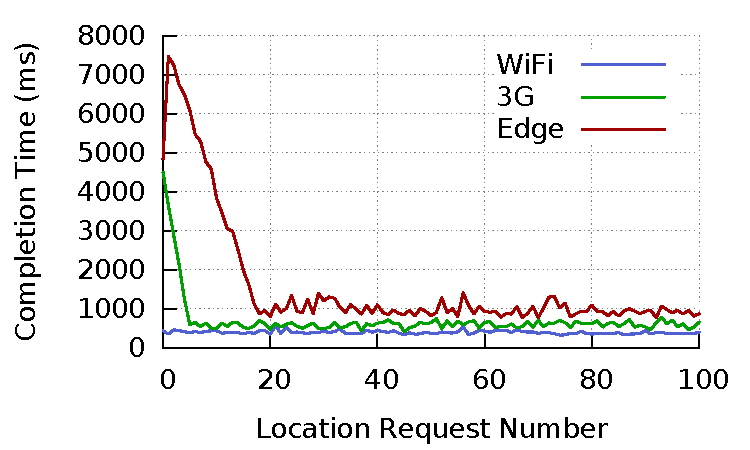
\includegraphics[width=.6\linewidth]{figures/phonesecures/tee_server_timed.pdf}
    \label{fig:ps_tee_synta}
  }
  
  \subfigure[] {%
    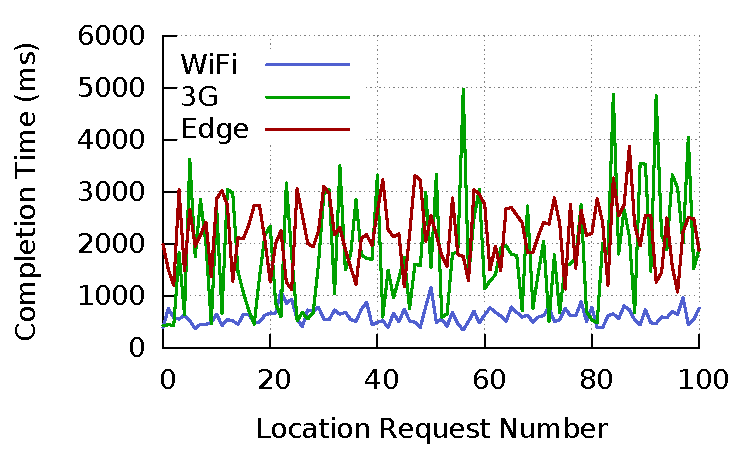
\includegraphics[width=.6\linewidth]{figures/phonesecures/tee_server_timed_secs.pdf}
    \label{fig:ps_tee_syntb}
  }
  \caption[Completion time for 100 location verifications]{Completion time for
  100 location verifications. In Figure (a) the server initiates one request
  per second. In Figure (b) the server waits 30 seconds before issuing each
  request.}
\end{figure}

Finally, Figure~\ref{fig:ps_tee_syntc} shows the average and the standard
deviation for the measurements of Figure~\ref{fig:ps_tee_syntb}. The completion
time for our solution is, on average, 2.2 seconds with an Edge connection, 1.82
seconds with a 3G connection, and 0.6 seconds with a WiFi connection,
respectively.

\begin{figure}[!ht]
  \centering
  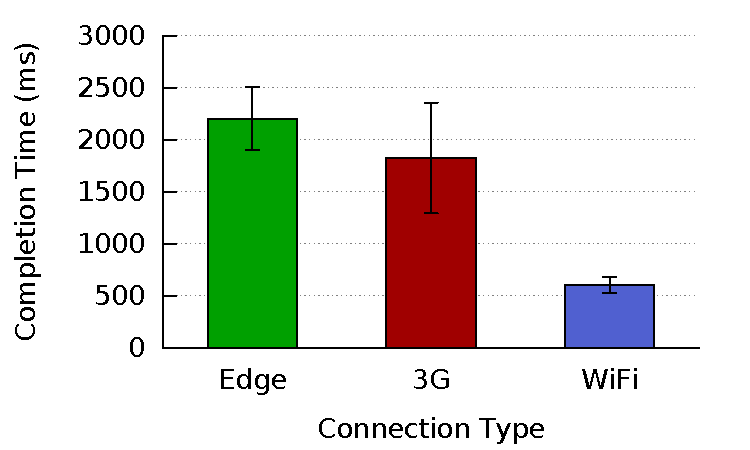
\includegraphics[width=.6\linewidth]{figures/phonesecures/tee_server_overview.pdf}
  \caption[Average time and standard deviation required to complete a location
  verification]{Average time and standard deviation required to complete a location
  verification, for different connection types.}
  \label{fig:ps_tee_syntc}
\end{figure}

\subsection{Field Study}

To test our solution in a setting close to the actual payment scenario, we use
two client devices and carry out a two-day field study with two subjects in
Z\"{u}rich.  Each subject carries a client device and a triggering device.  The
two clients have SIM cards issued by different operators (\emph{Orange} and
\emph{Sunrise}).

The triggering device initiates a server request. The server runs on a standard
laptop and listens for incoming triggers.  We use a separate trigger device to
make sure that, at the time of a location verification, the radio on the client
device is not active.  In an actual deployment, if the radio happens to be
active when a location verification request is received, completion time is
expected to be smaller than the ones reported below.

For two days, each subject uses the triggering device to initiate a location
verification each time he is close to a payment terminal in, for example, shops,
cafes, museums, parking lots, etc. Completion time, for the device with the
Orange SIM card, is 2.54 seconds on average (standard deviation 0.78
seconds). The smartphone with the Sunrise SIM card shows slightly worse
performance as the completion time raises to 3.68 seconds on average (standard
deviation 1.45 seconds).

Table~\ref{tab:ps_tee_citytab} shows the accuracy of the location information and the
elapsed time between the server request and the actual GPS fix on the client.
The reported accuracy is within an acceptable range to distinguish shops next to
each other (17.40 meters on average), and the location fix is available with a
very short delay (less than 257 milliseconds on average).

\begin{table}[!ht]
  \centering
  \small
  {\tabulinesep=.7mm
    \setlength{\tabcolsep}{1.2mm}
    \begin{tabu}{|ccc|ccc|}
      \hline
      \multicolumn{3}{|c|}{\textbf{GPS accuracy (m)}} &
      \multicolumn{3}{c|}{\textbf{GPS fix delay (ms)}}\\ \hline
      average & max & min & average & max & min\\
      17.40 & 48.0 & 4.0 & 256.83 & 3430.00 & 0.00\\ \hline
    \end{tabu}}
  \caption[Location accuracy results during the field study]{Location accuracy results during the field study.}
  \label{tab:ps_tee_citytab}
\end{table}

\section{Discussion}
\label{sec:ps_tee_discussion}

This section further discusses the proposed mechanisms in terms of integration
with current payment systems, deployment considerations, and privacy
issues. Finally, we discuss the applicability of our solution to other
scenarios.

\subsection{Integration with Payment Systems}

Our protocols can increase the security of any payment card transaction (either
``chip and PIN'' or ``swipe and sign'') where the card issuer is contacted by
the terminal to authorize or deny the payment.  We now detail the integration of
our solution with deployed payment systems and, in particular, with the EMV
payment standards~\cite{emv}.

An EMV transaction involves the card, the terminal, the card issuer and an
\emph{acquirer}. The acquirer is a banking institution that processes credit
and debit card payments for merchants. Third-party payment processors may be
also involved, or the issuer and the acquirer may be the same banking
institution. EMV specifications for transactions with online authorization
dictate two \emph{cryptograms} (authenticated messages) exchanged between the
card and its issuer. The cryptogram sent by the card is denoted as the
Application Request Cryptogram (ARQC) and accounts for a number of fields that
are supplied either by the card or by the terminal. Mandatory fields for ARQC
include the transaction amount, the transaction date, and a random nonce
generated by the terminal. EMV also defines optional fields that individual
payment systems (e.g., Mastercard M/Chip or Visa VSDC) may require. The card
issuer replies with an Application Reply Cryptogram (ARPC) that notifies the
card whether the transaction has been approved. Figure~\ref{fig:ps_tee_payment}
illustrates the messages defined in the EMV standards; dashed arrows show the
additional messages required to implement our solution.

\begin{figure}[!ht]
    \centering
    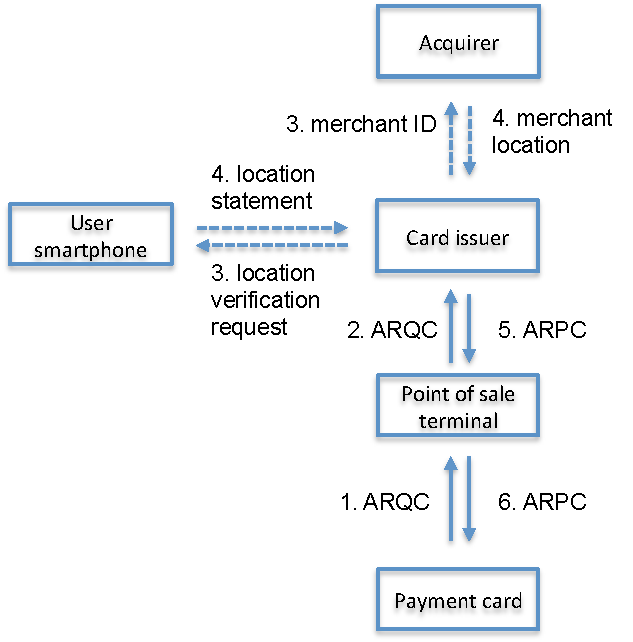
\includegraphics[width=0.7\linewidth]{figures/phonesecures/tee_integration}
    \caption[Integration of the location verification protocol within the EMV
    payment standards]{Integration of the location verification protocol
    within the EMV payment standards. Dashed lines indicate the additional
    messages required for our solution.}
    \label{fig:ps_tee_payment}
\end{figure}

Our solution requires the card issuer to know the physical location of the
terminal used for a transaction. In the EMV standards an \emph{acquirer ID}
globally identifies a banking institution, while a \emph{merchant ID}
identifies a merchant within a banking institution. Either the card or the
terminal can request that these elements are included in the ARQC message. Once
the card issuer learns the acquirer and merchant identifiers of a transaction,
it can contact the acquirer with the purported merchant ID in order to retrieve
the merchant location. Popular payment systems are already providing merchant
information, such as location, through standardized
APIs~\cite{mastercarddev,visadev}.

In current EMV payment systems, the acquirer ID and the merchant ID fields are
defined by the standard but are not mandatory for ARQC messages.  Through card
software updates it is possible to include these fields in ARQC messages of
every transaction.  The EMV standards allow for remote update of payment card
software through \emph{issuer scripts} that may be included in the ARPC
cryptogram.

A noteworthy benefit of our solution is that it enables gradual and secure
deployment for selected users. A card issuer can enable location verification
for a subset of its customers, for example, by updating the payment cards of
customers that decide to opt-in. Once location verification is enabled for these
users, an adversary that has obtained a payment card of any such user cannot
circumvent the system. In comparison, solutions that require gradual terminal
updates do not provide similar protection, as the adversary can always bypass
the added security mechanisms by utilizing not yet updated terminals.

\subsection{Deployment Considerations}

Even though fraud reduction is a clear incentive for banks or payment card
issuers to adopt our solution, it is the user adoption that will be the driving
factor. The proposed schemes do not change the user experience at points of
sale, but they do consume internet bandwidth and battery on the user's
device. Since payment card issuers are currently covering the costs of frauds,
it is an open question whether users would pay the additional costs in terms of
bandwidth and battery on their mobile devices, without any apparent benefit. To
boost the user adoption, the card issuer may offer lower fees to users who
opt-in, just like car insurance companies do for customers who install
anti-theft mechanisms on their cars.

Our solution assumes the user's smartphone to have Internet connectivity at the
time of a transaction.  This may not hold for two reasons.  First, high roaming
charges induce many users to turn Internet access off while traveling abroad.
International regulatory bodies have started to forbid excessive roaming
charges.  For example, the EU has recently decided to completely remove roaming
charges within its member countries by 2015~\cite{telegraph2013roaming}.  A
cost-effective alternative to avoid current roaming charges is to use SMS
messages for communication between the user's device and the card issuer.
SMS-based communication, can however experience high delays (SMS message
delivery is based on a best-effort basis and can take up to 12 seconds in normal
load conditions~\cite{smsdelay}). Second, Internet connectivity might not be
available in remote areas or underground locations (although many underground
shopping centers or transport stations have cellular coverage).

Card issuers can handle lack of connectivity based on transaction value,
merchant location or user specific policies. For example, high-value
transactions in areas where Internet connectivity is expected to be available
may only be authorized after a successful location verification with the user's
smartphone. A possible solution to handle temporary lack of connectivity for
low-value transactions could be to keep, on the device, an authenticated log of
timestamped locations and report the one that is closest to the transaction
time, once Internet connectivity is again available.  While this solution does
not allow for real-time fraud prevention, it allows card issuers to perform
offline fraud detection.

\subsection{Privacy Considerations}

The card issuer can ask the user's device for location statements and track the
user over time.  However, if the protocol is triggered at times of genuine
transactions, our solution does not leak extra information, since the
card-terminal transaction already reveals the user location to the card
issuer. The card issuer may also abuse the system and query the user's device
for a location statement when the card is not involved in a transaction.  We
argue that the system abuse can be prevented through precise terms of agreement;
card issuers that break those terms will damage their reputation and lose
customers.  Another solution is to let the card issuer send the location of the
point of sale terminal to the device and let the device compare it against its
current location, as done in~\cite{park09acsac}.

With respect to third-parties (i.e., law-enforcement authorities), location
statements issued by the user's device can be denied.  Since the (symmetric)
service key used to authenticate location statements is shared with the card
issuer, no third-party can identify who produced a location statement (either
the user's device or the card issuer). Finally, we remark that an adversary in
control of the mobile OS on the victim's device can query the GPS unit at will
and track the user, independently of the solution presented in this chapter.

\subsection{Other Application Scenarios}

Our protocols can be applied to other application scenarios beside payments at
points of sale.  In particular, they can be used in any scenario where the
verifying party (e.g., a service provider) knows the user's phone number and the
location of the infrastructure used to perform transactions.  Two prominent
examples are public transportation ticketing and building access.

In the public transportation scenario the user holds a transport ticket (e.g.,
an NFC card) that is used at dedicated machines to access the transportation
network (e.g., at the entrance of metro stations). Our solution can provide
assurance to the public transportation authority that a lost or stolen transport
ticket is not used by any party but the rightful owner.

Similarly, building access control systems require a user to carry an access
token with a short-range wireless interface. Entry is granted if the token is
presented to a dedicated reader and the valid PIN is entered by the user.
Location statements can increase the security of such access control systems.
Upon presenting the access token to the reader, the user phone is queried for
its location; if the purported location matches the one of the reader, the
building access authority can grant access.

As part of our field study (described in Section~\ref{sec:ps_tee_experimental}), we
tested completion time and accuracy of our location verification protocol in
public transportation and building entrance scenarios. Results are summarized in
Table~\ref{tab:ps_tee_completionothers} and Table~\ref{tab:ps_tee_accuracy}.

Completion time at public transport stations takes 3.03 seconds on average,
using a 3G connection, for the device using Orange, and 3.39 seconds on average
for the smartphone using Sunrise. We argue that three seconds to grant access
to the transportation network may be an undesirable delay. Nevertheless, our
solution could be used for offline ticket abuse monitoring. The public
transportation authority could disable a ticket after witnessing a number of
consecutive fraudulent uses. In this scenario, the measured location accuracy
(see Table~\ref{tab:ps_tee_accuracy}) is around 14 meters on average. In most
public transportation applications this accuracy is sufficient to distinguish
entrances to the transportation network from one another.

\begin{table}[!ht]
\centering
\small
{\tabulinesep=.7mm
    \setlength{\tabcolsep}{1.2mm}
    \begin{tabu}{|l|ccc|ccc|}
      \hline
	  \multicolumn{1}{|c|}{\textbf{Scenario}} &
      \multicolumn{3}{c|}{\textbf{GPS accuracy (m)}} &
      \multicolumn{3}{c|}{\textbf{GPS fix delay (ms)}}\\ \hline
      & avg & max & min & avg & max & min\\ \hline
      \footnotesize Building access & 14.04 & 48.0 & 4.0 & 139.31 & 3087.00 & 0.00\\ \hline
	  \footnotesize Public transport & 15.47 & 48.0 & 6.0 & 210.52 & 4035 & 0.00 \\ \hline
    \end{tabu}}
  \caption[Location accuracy for public transport and building access tests]{Location accuracy for public transport and building access tests.}
  \label{tab:ps_tee_accuracy}
\end{table}

We also test the time it takes to run our protocol when entering buildings in
two campuses of ETH Zurich, one in the city center and the other in the city
suburbs. Completion time takes 2.31 and 4.40 seconds on average, depending on
the network operator used as shown in Table~\ref{tab:ps_tee_completionothers}.
The location accuracy in this scenario is around 15 meters, which is enough to
differentiate building doors from each other in most cases.

\begin{table}[!ht]
\centering
\small
{\tabulinesep=.7mm
\setlength{\tabcolsep}{1.2mm}
\begin{tabu}{l|cc|cc|}
	\cline{2-5}
	& \multicolumn{2}{c|}{\textbf{Building access}} & \multicolumn{2}{c|}{\textbf{Public transport}} \\ \cline{2-5}
	& Orange & Sunrise & Orange & Sunrise \\
	& (n=59) & (n=40) & (n=43) & (n=63) \\ \hline
	\multicolumn{1}{|l|}{average (sec)} & 2.31 & 4.40 & 3.03 & 3.39 \\
	\multicolumn{1}{|l|}{std dev (sec)} & 0.57 & 1.74 & 0.66 & 1.33 \\ \hline
\end{tabu}}
\caption[Completion time for location verification for public transport and
building access tests]{Completion time for location verification for public
transport and building access tests. \emph{n} denotes the number of samples in
each scenario.}
\label{tab:ps_tee_completionothers}
\end{table}

\section{Alternative Approaches}
\label{sec:ps_tee_alternatives}

In this section we discuss alternative ways in which smartphones could provide a
second authentication factor for payments at points of sale, and conclude that
location verification provides a practical means for card issuers to identify
fraudulent transactions. We also analyze commonly suggested enrollment schemes
and show how they fail to provide secure user-to-device binding, given our
realistic attacker model. Finally, we describe alternative TEEs available on
current smartphones and their shortcomings, compared to system-wide TEEs such as
ARM TrustZone.

\subsection{Two-factor Authentication Approaches}
\label{sec:ps_tee_second-factor}

\begin{figure}[!ht]
  \centering
  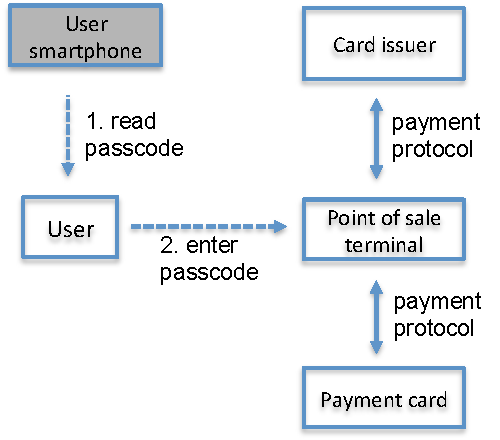
\includegraphics[width=.5\linewidth]{figures/phonesecures/tee_second-factor-A}
  \caption[Smartphone as an authentication token replacement]{\emph{Smartphone
  as an authentication token replacement:} the user reads a passcode off his
  smartphone and enters it into the payment terminal. Solid arrows represent
  standard transaction messages, while dashed arrows show additional messages
  for two-factor authentication.}
  \label{fig:ps_tee_second-factor-A}
\end{figure}

In a typical transaction at a point of sale, the user enters or swipes his
payment card into a terminal and optionally types its PIN code. The card runs a
protocol with the terminal that contacts the card issuer for online transaction
verification. We present common
two-factor authentication approaches: \emph{(1) Authentication token
replacement (Figure~\ref{fig:ps_tee_second-factor-A}).} The smartphone acts as
a dedicated authentication token and displays one-time passcodes that the user
must type into the terminal. Google 2-Step
Verification~\cite{google_authentication} is a prominent example of this
approach in the context of web login authentication. A similar approach can be
applied to payments at points of sale. \emph{(2) User confirmation device
(Figure~\ref{fig:ps_tee_second-factor-B}).} The card issuer contacts the user's
device which presents a confirmation dialog to the user. The confirmation
result is sent back to the card issuer. Authentication solutions like this one
have already been deployed for online banking~\cite{validsoft}. \emph{(3)
Distance-verification device} (Figure~\ref{fig:ps_tee_second-factor-C}). The
user places his smartphone next to the payment terminal, which starts a
distance-verification protocol over a short-range wireless connection, such as
NFC~\cite{googlewallet}.

\begin{figure}[!ht]
  \centering
  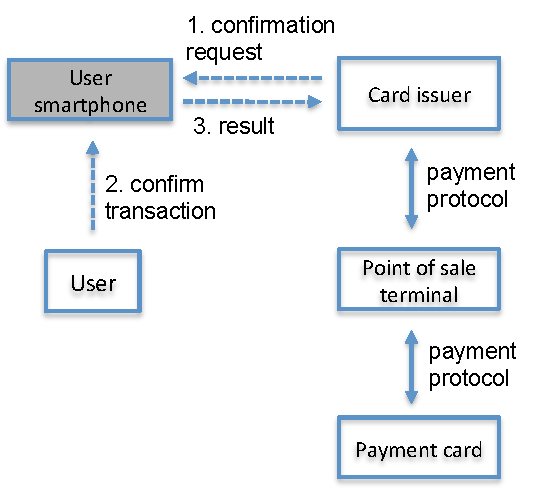
\includegraphics[width=.5\linewidth]{figures/phonesecures/tee_second-factor-B}
  \caption[Smartphone as a user confirmation device]{\emph{Smartphone as a user
  confirmation device:} the user confirms the transaction using his smartphone;
  the devices delivers the user's decision to card issuer. Solid arrows
  represent standard transaction messages, while dashed arrows show additional
  messages for two-factor authentication.}
  \label{fig:ps_tee_second-factor-B}
\end{figure}

\begin{figure}[!ht]
  \centering
  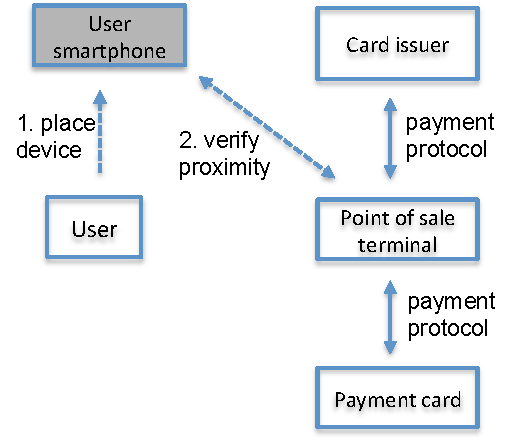
\includegraphics[width=.5\linewidth]{figures/phonesecures/tee_second-factor-C}
  \caption[Smartphone as a distance verification device]{\emph{Smartphone as a distance verification device:}  the user positions the phone next to the terminal; the terminal verifies the proximity of the phone over short-range wireless connection (e.g, NFC). Solid arrows represent
  standard transaction messages, while dashed arrows show additional messages
  for two-factor authentication.}
  \label{fig:ps_tee_second-factor-C}
\end{figure}

The given approaches require additional user interaction at the time of the
transaction. Changes to established user interaction models hinder the
introduction of new security mechanisms~\cite{bonneau12sp}. Additionally, the
majority of point of sale terminals do not have the required software
components for passcode entry (Figure~\ref{fig:ps_tee_second-factor-A}) or
hardware interfaces for distance-verification
(Figure~\ref{fig:ps_tee_second-factor-C}). The replacement of deployed
terminals would be gradual and optional, which allows the adversary to target
the terminals that have not been updated yet.

\subsection{Common Enrollment Solutions}
\label{sec:ps_tee_straightforward}

We now explain why commonly suggested enrollment schemes are not secure or
feasible to deploy, assuming an adversary that controls the mobile OS on the
victim's device.

\paragraph{Device Identifier Enrollment.}

A simple way to bind a user identity to the device key of his TEE, is to
leverage the device's IMEI, typically included in the device certificate.  The
IMEI is available on the device's package or displayed on-screen.  During
enrollment, the user provides the IMEI of his device to the card issuer using a
reliable out-of-band channel, for example, visiting a branch of the card issuer
in person. The card issuer then verifies the device certificate with respect to
the IMEI provided by the user.

Communicating the IMEI to the card issuer in a trustworthy way is more
complicated than it seems.  Device sales packages are not always available.
Also, if the mobile OS is compromised, the adversary controls the IMEI shown on
the device screen.  Additionally, IMEI-based enrollment does not provide
flexible device migration: every time the user changes devices, he must provide
the IMEI of the new device to the card issuer, using an out-of-band channel.

\paragraph{Password Enrollment.}

The user-to-device binding can also be implemented by asking the user to enter a
password or a similar initialization secret, known by the card issuer, in his
device.  A trusted application can authenticate itself to the card issuer, using
the certified device key and the user-provided password.

The user should type in the password only when a trusted application can
securely receive it. The compromised mobile OS can otherwise intercept and
forward the password to the adversary, who can then launch an impersonation
attack. A reliable communication interface from the user to a trusted
application is called \emph{trusted path}~\cite{yee2002icics, ye2005tissec}. The
device hardware and software resources used for user interaction (e.g., the
display buffer or the touchscreen input events) can be temporarily reserved for
system-wide TEEs such as ARM TrustZone.  A \emph{security indicator}, such as a
colored bar on the top of the screen~\cite{selhorst10trust} or a dedicated
LED~\cite{armTZslides} can be used to inform the user about the type of
application he is communicating with (trusted or untrusted). However, current
smartphones do not support this division of user interface resources, nor do
they provide dedicated security indicators. Furthermore, several academic
studies, and a few decades of practical experience, have shown that users tend
to ignore security indicators~\cite{schechter07sp, egelman2008chi,
  jackson2007usec}.

Previous work assumes that password-based enrollment is secure if the enrollment
is done early in the device lifecycle, before the adversary has the opportunity
to compromise the mobile OS~\cite{czeskis12ccs,kari11stc}. This assumption is
hard to justify since not every service enrollment happens at the beginning of a
device life time.

\paragraph{SMS Enrollment.}

If the user provides his phone number during registration, the card issuer can
send an SMS message that will be received by the device in which the user's SIM
card is installed. Similarly to our solution, the SMS message could carry an
initialization secret to bootstrap security services. The problem with this
approach is that SMS messages provide a trustworthy channel to the the baseband
OS of the device where the SIM card is installed, but not to the secure world on
that device.  In current mobile device architectures, the baseband OS is
accessible by both the mobile OS in the normal word and by the trusted
applications running in the secure world. Therefore, when the baseband OS
receives an SMS message, it notifies the mobile OS, which can read any
initialization secret and leak it to the attacker. Assuming a mobile device
architecture in which the baseband OS interacts only with the secure world is
not feasible, as the mobile OS needs to interact with the baseband for, e.g.,
phone calls. To overcome this limitations, the baseband-assisted enrollment
scheme uses an enhanced baseband OS to achieve secure enrollment.

\paragraph{Enrollment Using Initialization Secrets.}

Figure~\ref{fig:ps_tee_channels} illustrates the user enrollment problem when
using initialization secrets. Any channel to the secure world can be
intercepted by the mobile OS in the normal world, be it the baseband OS, the
user-interface, or any other interface such as NFC or Bluetooth. For example,
the baseband OS cannot pass the initialization secret received over SMS
messages to the application processor because it does not know which processor
state (normal world or secure world) is active.

\begin{figure}[!t]
    \centering
    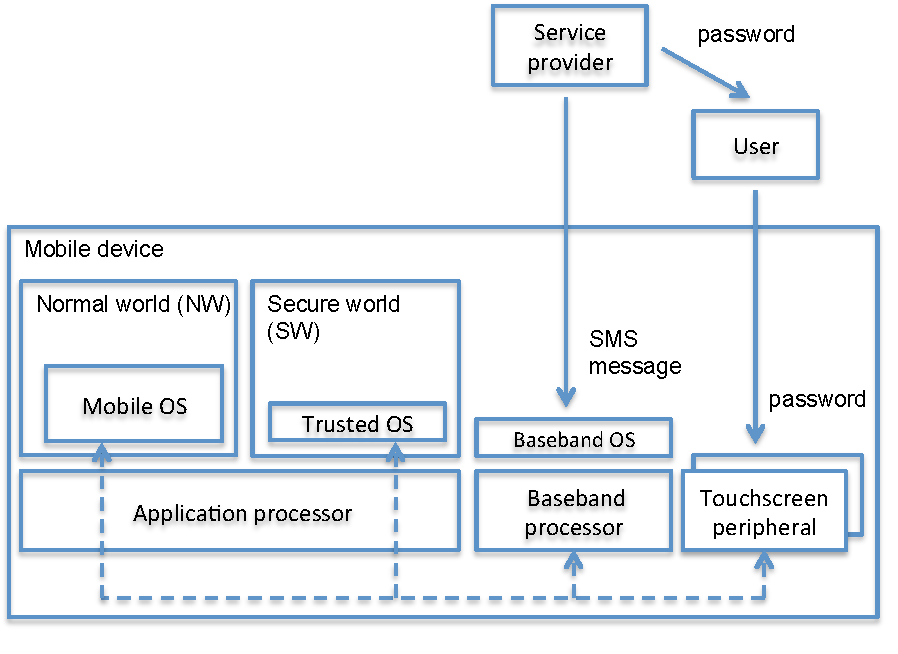
\includegraphics[width=.8\linewidth]{figures/phonesecures/tee_channels2}
    \caption[Commonly suggested user enrollment schemes]{Commonly suggested
    user enrollment schemes. Solid arrows illustrate trustworthy communication
    channels. Dashed arrows illustrate communication channels in which one of
    the end points can be either the normal world or the secure world.}
    \label{fig:ps_tee_channels}
\end{figure}

\subsection{Alternative Trusted Execution Environments}

In addition to ARM TrustZone, SIM cards are TEEs widely available on
smartphones. A SIM card can store secrets and execute small pieces of code
(often referred to as \emph{SIM applications}) in isolation from the mobile OS.
Therefore, one could argue that the location verification mechanism can be
implemented as a SIM application within the SIM card processing environment.
This approach has two drawbacks. First, provisioning of SIM applications to a
SIM card requires the service provider to negotiate with the network operator
that issued that SIM card. Providers who target global applications must
negotiate with a large number of network operators separately. Second, in
current architectures, SIM cards cannot directly access the device peripherals,
such as the GPS unit. When the SIM card needs location information, the
application processor must read the coordinates from the GPS unit and provide
them to the SIM card. The SIM application has no means of knowing whether these
coordinates have been tampered with. Some recent device configurations support
a dedicated connection between the SIM card and the device NFC
unit~\cite{gsma2011}. Similar dedicated lines could be added for secure access
to the GPS unit. However, targeted hardware changes to allow for specific
security services based on SIM applications are costly and hard to justify for
widespread adoption.

Some mobile devices are equipped with a slot for SD cards. The latter may be
used as a TEE to run code in isolation from the mobile OS or to securely store
credentials~\cite{gdsdcard,smartSD}. However, just like SIM cards, SD cards do
not have direct access to the device peripherals, such as the GPS unit, and
remote provisioning of applications by third-parties to SD cards is not
currently available.

\section{Related Work}

In chapter~\ref{chap:ps_relatedwork} we discussed  alternative approaches to 2FA also in the context of payments. In the following we review related work that focuses on secure enrollment and trusted execution environments for smartphones.

\noindent\emph{Secure Enrollment.}
Secure enrollment for trusted platforms~\cite{parno_trust} and TEEs on mobile
devices~\cite{2013_spsm_marforio} is a challenging research problem. Both
deployed systems~\cite{barclays_pinsentry,google_authentication} and academic
work~\cite{park09acsac,liu12mobisys,gilbert11sensys} have overlooked it or
assume a non-compromised OS at enrollment time~\cite{czeskis12ccs,kari11stc}.

In~\cite{tz-secondfactor} the authors evaluate how TrustZone-enabled
devices can substitute hardware tokens for two-factor authentication. They
assume a trusted path to the user for which secure implementation is problematic.
In~\cite{vasudevan12trust} the authors systematize hardware-based
solutions that increase the security guarantees available on mobile
platforms. In their work the authors do not address the problem of secure
enrollment.
Even in recent work that proposes the use of mobile TEEs for security-critical applications~\cite{busold2013codaspy,dmitrienko2011trust,tamrakar2013trust}, 
the problem of secure enrollment is not addressed.

\noindent\emph{Trusted Sensors.}
Saroiu and Wolman~\cite{sariou10hotmobile} put forward the problem of
trustworthy sensor readings on mobile phones. They propose to leverage
virtualization to handle sensors readings and provide signed measurements to
applications that run in guest VMs.  A similar approach is considered
in~\cite{gilbert10hotmobile} where the authors consider participatory sensing
scenarios and study how to protect user privacy and how to allow for local data
processing while providing (TPM) signed sensor readings.  Trustworthy
participatory sensing applications are also considered in~\cite{dua10hotsec},
where the authors design and implement a trusted sensing platform. The latter is
a board equipped with sensors and a TPM that communicates with the mobile device
over Bluetooth and provides signed sensor measurements.

Liu et al.~\cite{liu12mobisys} build on top of Credo~\cite{credo} and TrustZone
to propose software abstractions that expose trusted sensor services to mobile
applications. In particular, the authors of~\cite{liu12mobisys} focus on scenarios where
trustworthy reading must be processed locally by applications (e.g., blurring
people's faces from a photo taken by the phone's camera) before being
sent. Therefore the framework in~\cite{liu12mobisys} aims at protecting the
integrity of a sensor reading as well as the local code that must process it.
The authors provide a sample application scenario where sensor readings account
for GPS traces, while data processing applies noise to the aggregated outcome in
order to achieve differential privacy~\cite{dwork06icapl}.

Plug-n-Trust~\cite{sorber12mobisys} focuses on mHealth scenarios and provides a
system to protect integrity and confidentiality of data collected by body-area
network of sensors.  Their approach leverages a smart card that plugs into a
phone's microSD slot and creates a trusted computing environment for collecting
and processing data provided by surrounding sensors.  Security rests upon tamper
resistance of both the smart card and the sensor nodes where
encryption/authentication keys are stored.

YouProve~\cite{gilbert11sensys} addresses scenarios where sensor readings must
be modified by local applications for, e.g., privacy issues. The authors
of~\cite{gilbert11sensys} propose a framework to verify that a modified data
item preserves the meaning of the original sensor reading.  YouProve uses
TaintDroid~\cite{taintdroid} to track the measurement from the moment it is
produced by the sensor, until the moment it is uploaded to a service provider.
Each modification is tracked, and a summary of all changes is signed using the
secret key of the phone's TPM.

To the best of our knowledge, all previous work on trusted sensors focuses on
designing or developing a trusted computing environment on a mobile device in
order to cryptographically sign sensor readings. However, these work do not
address secure deployment aspects, including secure enrollment and device
migration. To the best of our knowledge, we are the first to propose a complete
and deployable solution that allows a number of application scenarios to
leverage on-smartphone trusted sensor measurements.

\section{Summary and Future Work}

As we have seen in the context of web applications, two-factor authentication plays an important role in securing users' accounts and data. In this chapter we have further shown how this extends to other scenarios. In particular we focused our attention to providing a solution that can thwart fraudulent transactions at points of sale.

We proposed a practical solution that adds the required security to recently proposed location-based two-factor authentication mechanisms. We have identified the necessary requirements for a deployable solution, which includes no changes to the user experience and to the infrastructure that is already in place. We have proposed a new mechanism to secure the readings of the smartphone GPS sensor in order to strengthen the security of our solution. Furthermore, we have proposed two novel enrollment schemes that enable secure enrollment and convenient device migration despite a compromised mobile OS. With these solutions we can protect customers transactions at points of sale even in the presence of a motivated adversary that performs targeted attacks against a particular user. Through prototype implementations on current hardware we have shown that our solution is indeed deployable. We further tested the proposed location-based mechanism in a field study and showed that the location verification operations causes an acceptable delay during a payment transaction. Finally, we presented other use-cases where our solution can be used to enhance their security such as entrance to buildings and ticketing.

\subsection{Future Work}

In this chapter we presented a solution to strengthen the security of payments at points of sale. We now look at future research directions.

\paragraph{TrustZone Implementation.} As part of our work we presented prototype implementations that allowed us to showcase the feasibility and deployability of our proposed solutions. Unfortunately, at the time of this writing, it was not possible for us to fully implement the proposed security mechanisms on a standalone device. We believe that an open platform that allows deployment of applications in the secure world of TrustZone-enabled smartphones will enable a better understanding of all the intricacies of the work presented in this chapter. Such research would also provide a strong proof that our work indeed satisfies not only the security but also the timing and usability requirements of our solution.

\paragraph{Terminals Location.} The assumption we made in this chapter is that the location of payment terminals is known in advance by the service provider that makes the location comparison. In cases where the terminals location is unknown, our proposed solution cannot be deployed. We believe that one could carry out a study on the accuracy of the location information of payment terminals. Furthermore, it is possible that within an organization (e.g., a supermarket chain) payment terminals are moved between different locations due to renovations or relocations. It would be interesting to understand how often this happens and how many false negatives would be generated by such a move if the database is not promptly updated. One could further propose solutions to crowd-source the data in cases where the terminals are moved or the location data is missing. Such a solution would have to take into account an attack window while the data is crowd-sourced. Furthermore, it would be interesting to understand how fast the terminal locations can be successfully crowd-sourced depending on the payments distribution among multiple terminals.


